\documentclass[12pt, twoside]{article}
\usepackage[francais]{babel}
\usepackage[T1]{fontenc}
\usepackage[latin1]{inputenc}
\usepackage[left=1cm, right=1cm, top=1cm, bottom=1cm]{geometry}
\usepackage{float}
\usepackage{graphicx}
\usepackage{array}
\usepackage{multirow}
\usepackage{amsmath,amssymb,mathrsfs}
\usepackage{soul}
\pagestyle{empty}

\begin{document}


\section*{\center{Un partage �quitable}}
\begin{tabular}{cc}
\begin{minipage}{7cm}
\begin{center}
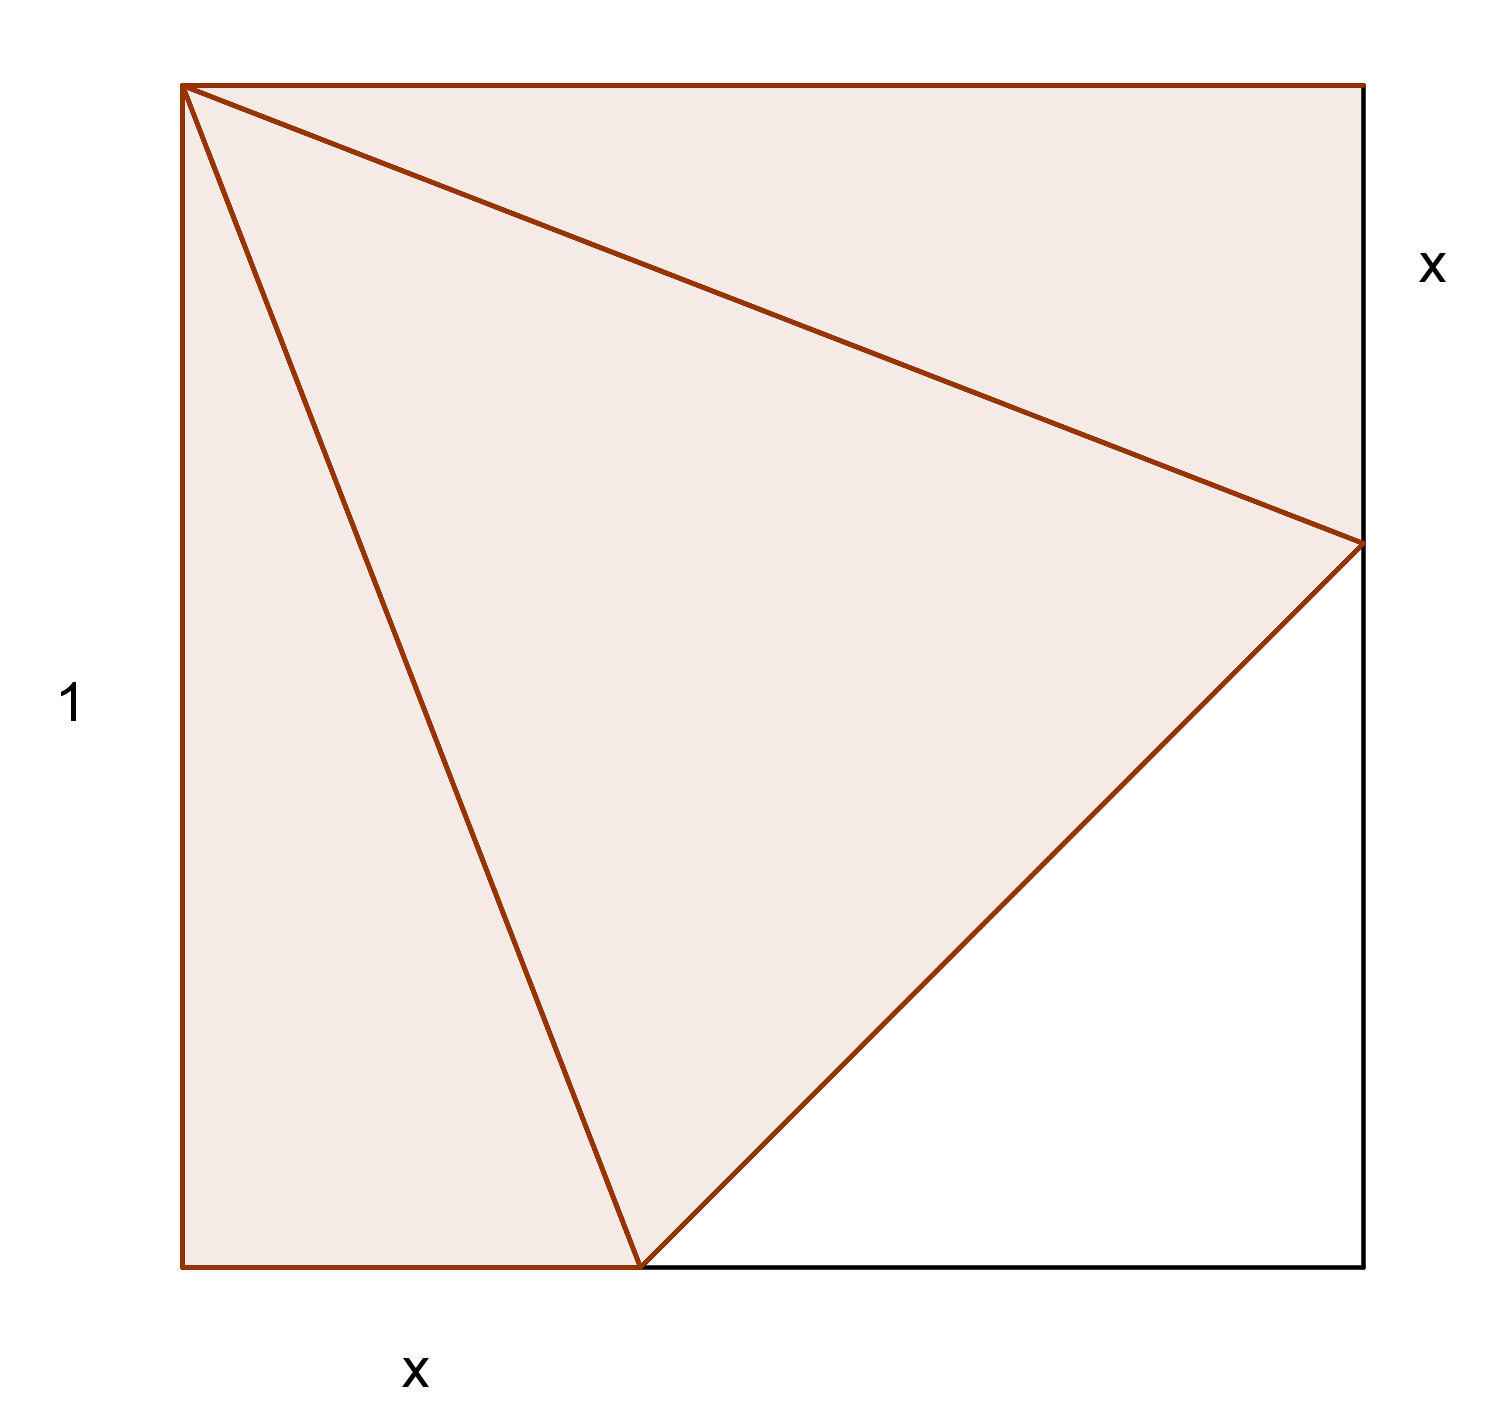
\includegraphics[width=5cm]{image/aer3.png}
\end{center}
\end{minipage}
&
\begin{minipage}{9cm}
L�onard est g�om�tre. Il veut partager un carr� de c�t� 1 selon le sch�ma
suivant. Il souhaite que les 3 triangles color�s soient de m�me aire. Quelle
valeur doit-il donner � x pour arriver � ses fins?
\end{minipage}
\end{tabular}


\bigskip
\bigskip


\section*{\center{Un partage �quitable}}
\begin{tabular}{cc}
\begin{minipage}{7cm}
\begin{center}
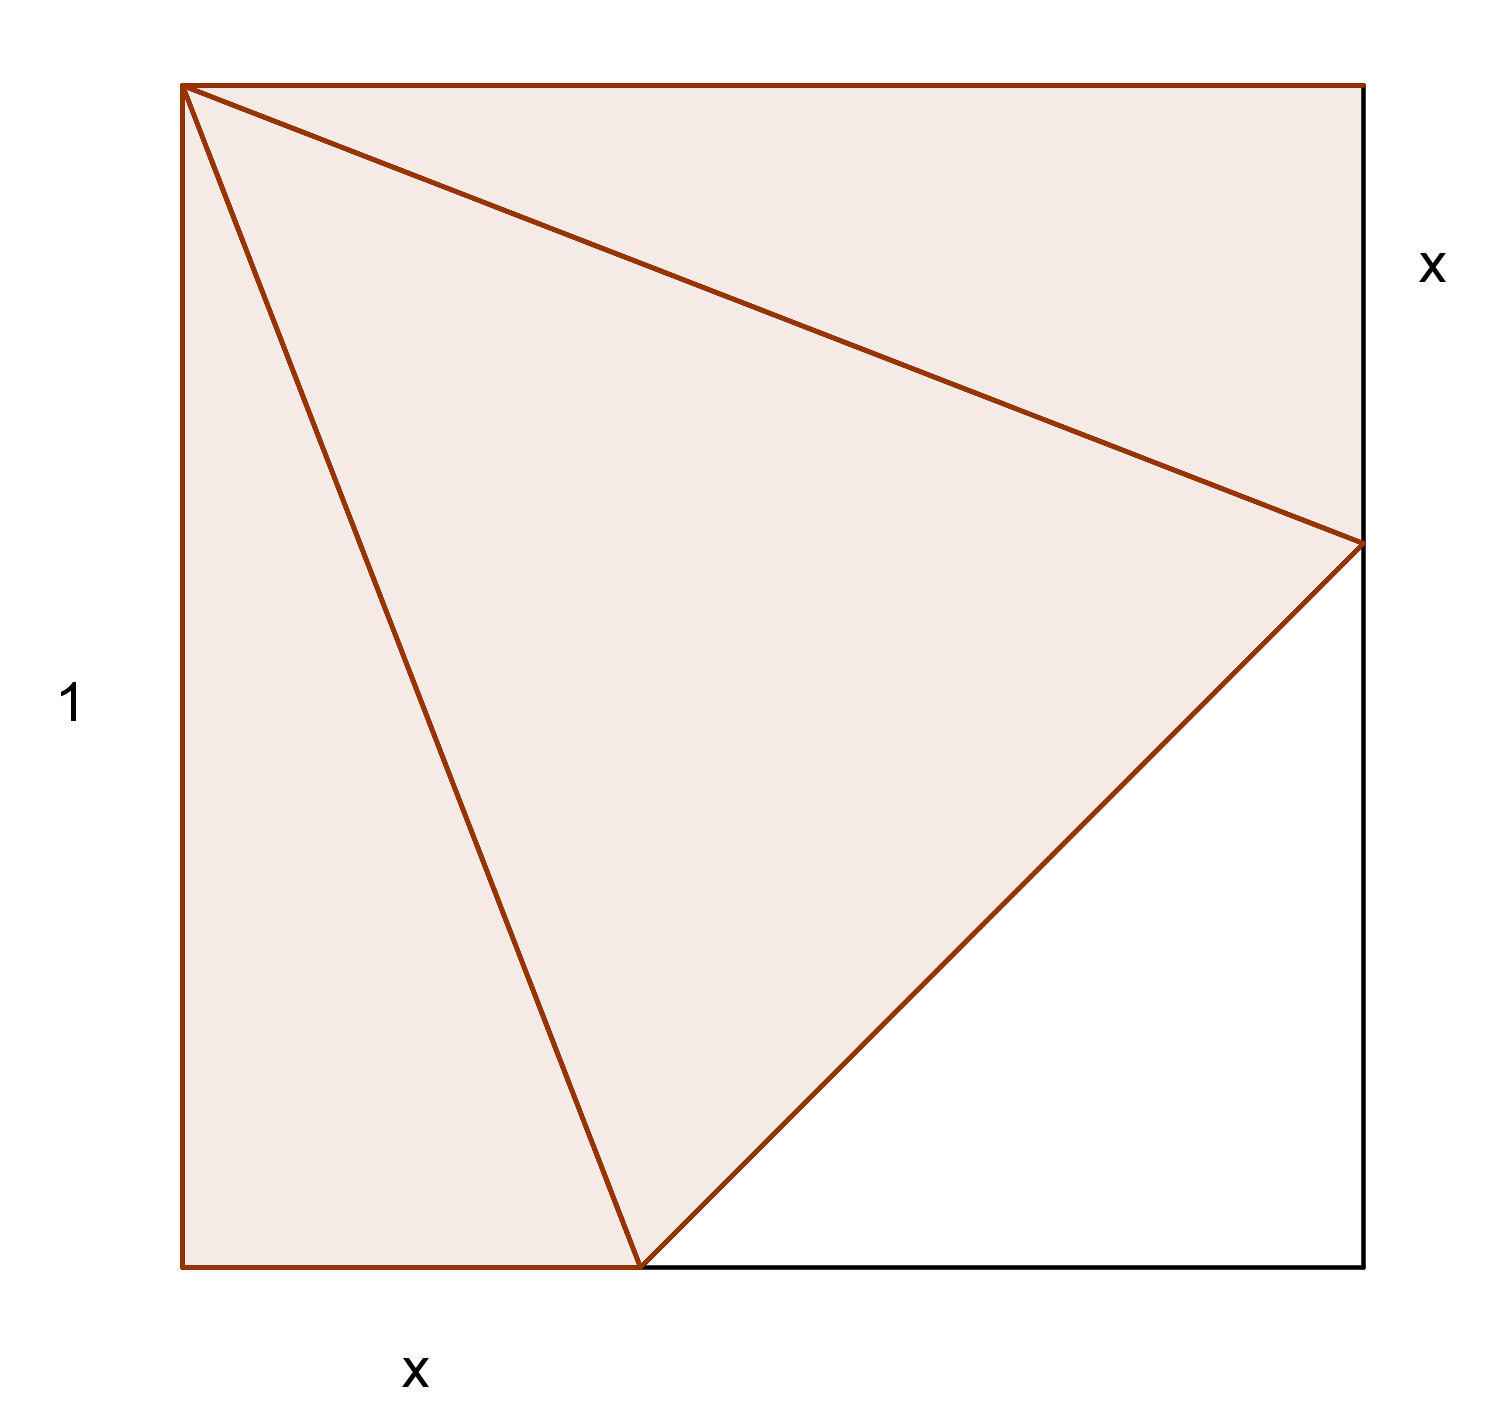
\includegraphics[width=5cm]{image/aer3.png}
\end{center}
\end{minipage}
&
\begin{minipage}{9cm}
L�onard est g�om�tre. Il veut partager un carr� de c�t� 1 selon le sch�ma
suivant. Il souhaite que les 3 triangles color�s soient de m�me aire. Quelle
valeur doit-il donner � x pour arriver � ses fins?
\end{minipage}
\end{tabular} 

\bigskip
\bigskip


\section*{\center{Un partage �quitable}}
\begin{tabular}{cc}
\begin{minipage}{7cm}
\begin{center}
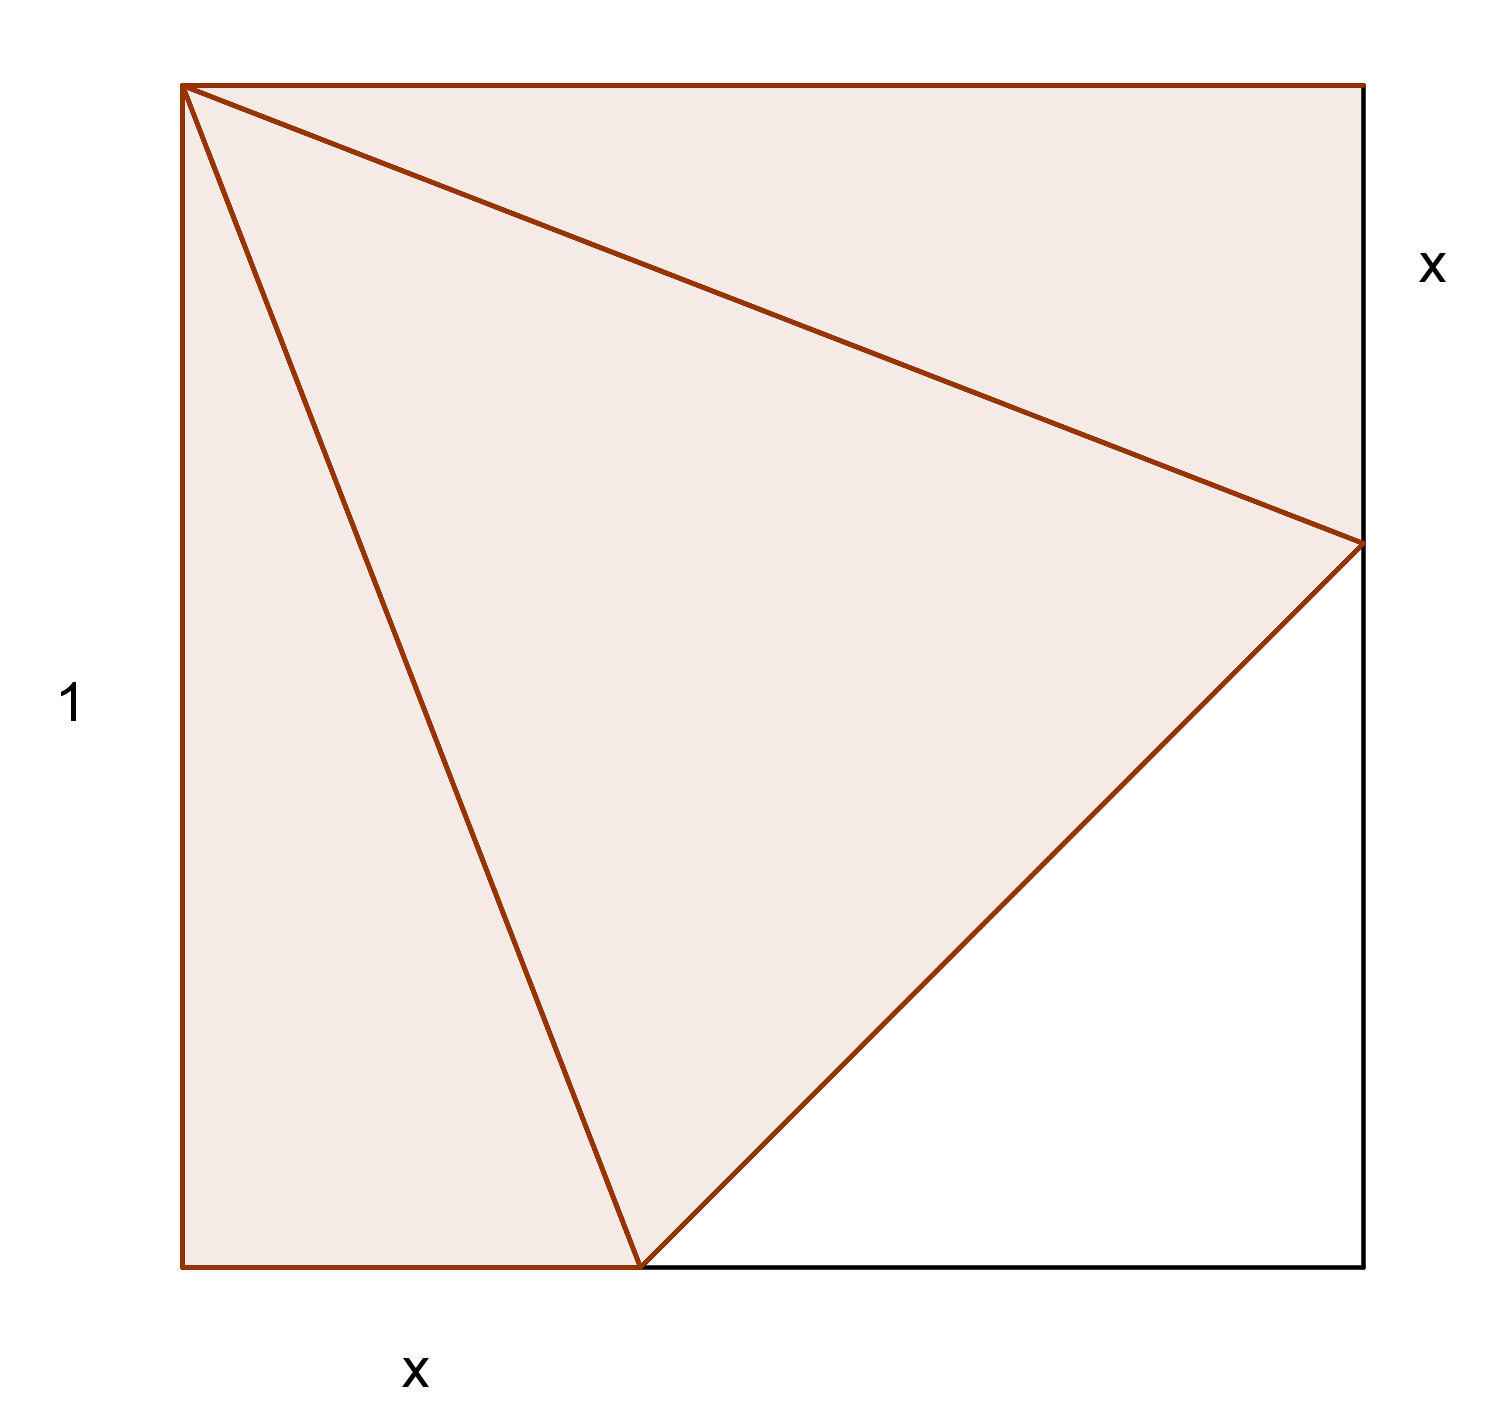
\includegraphics[width=5cm]{image/aer3.png}
\end{center}
\end{minipage}
&
\begin{minipage}{9cm}
L�onard est g�om�tre. Il veut partager un carr� de c�t� 1 selon le sch�ma
suivant. Il souhaite que les 3 triangles color�s soient de m�me aire. Quelle
valeur doit-il donner � x pour arriver � ses fins?
\end{minipage}
\end{tabular}


\end{document}
